\chapter{Security} 
\label{Security}

\lhead{Chapter X. \emph{Security}}

In this chapter we will discuss the security in our implementation of NIPEN.
We will also talk about what type of security would be expected in a final implementaion of NIPEN. There will also be a short mention of HIPAA and what role that act will play in a system like this.

\section{Security in our solution}
We cleared it with the customer earlie that to make it easy and achievable for us to make this proof of concept we had to skip most of the security needed.
Therefor the data used is not encrypted. 
We are only using Hypertext Transfer Protocol (HTTP) for transportation of data and not using the Secure Socket Layer (SSL).  
We have also not implemented an authentication system.
Since we have not implemented an authentication system there is only one user of the system.
Every user of the system has access to that users data.

\section{Security in NIPEN}

In this section we will discuss some of the factors that should be considerd when implementing NIPEN on a large scale.
We will breefly cover HIPAA and the different forms of security needed for this type of system like authentication, storage and trasportation of the data.


\subsection{HIPAA - Health Insurance Portability and Accountability Act}

After discussing security with the customer we brought up the topic of HIPAA \cite{HIPAA}. 
Even though there are no similar act in Norway the customer belived that taking a starting point from HIPAA to discuss the security in NIPEN would be a smart basis. 

\subsection{Storage of data}
When the data is at rest the network should be protected from intusions.
The hard drives where the data is stored must be encrypted. \cite{Encryption}
HIPAA dose not specify what type of encryption should be used they only specify that it should be encrypted.

\begin{figure}[H]
\centering
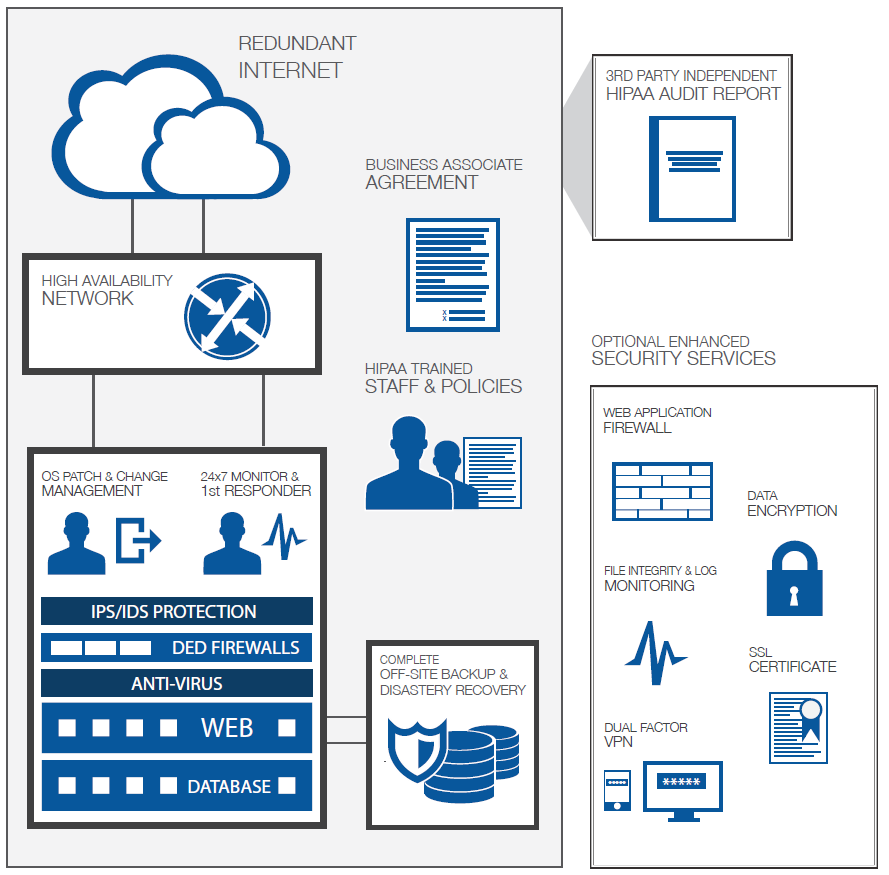
\includegraphics[scale=0.50]{../Figures/hipaa.png}
\caption{HIPAA Compliant Data Center Architecture from www.onlinetech.com}
\label{figure:HIPAA}
\end{figure}


\subsection{Transportation of data}
In HIPAA the transportation of data is described that it needs to use Secure Socket Layer. 
This layer is designed to give communication security over the Internet. cite{SSL}


\subsection{Authentication}
There are multiple systems already in use today in Norway for authenticating users. 
Some of the biggest systems are MinId, BankID, Buypass and Commfides.
The most widespread right now is BankId, with almost 3 million users as of this writing (https://www.bankid.no/).
It would be worth a consideration to use BankID to authenticate the citizens. 
The reason behind this is that it is a widespread system and sometihng the citizens are familier with. 

When considering what type of authentication the medical professionals should use there are multiple factors to consider. 
Ease of use, efficienty and be able to make an audit trail are som extra factors too consider.
It might be as succesfull to develope a seperate system of authenticating the health professionals if BankID turns out to be cumbersum and unable to be used in the different situations needed for this system. 
For HIPAA there needs to be a system to know which information was accessed, when, and by whom. \cite{Audit}

\subsection{Giving data to third party systems}
Not only should this system accept data from third parties. 
There should also be functionality for exporting data from the system to third party providers. 
For this to happen there needs to be a system for the end users, the citizens, to understand where and to whom the data is going.
Any data that is Protected Health Information \cite{PHI}, whitch is defined as any data classified as health information connected by the patients identifiers, the end user must controll how this information is shared. 
In the end its up to the user who they want to share their data with.
What could be smart is to introduce a Norwegian sertification so that the end user knows that the data providers they want to export their data to follows the roules mentiond in previous subsections. 
That way it is easier for the user to trust new systems with their sensitive data.
